\documentclass{jfm}

% Compilation
\usepackage{silence} % Silence latex compiler warnings
\WarningFilter{latex}{Command \@xhline has changed} % Filter out warning
  % caused by redefinition between jfm.cls class and array (loaded by
  % siunitx)

% Import custom style file containing common packages and options
\setlength{\paperheight}{\pdfpageheight} % JFM class removes paperheight definition and hyperref raises a warning

% Import custom style file containing common packages and options
\usepackage{preamble}
\graphicspath{{./Figures/}}

% Discrete Fourier Transform
\newcommand{\GenP}{\hat{P}_m}
\newcommand{\POne}{\hat{P}_1}
\newcommand{\PTwo}{\hat{P}_2}
\newcommand{\PThree}{\hat{P}_3}
\newcommand{\PFour}{\hat{P}_4}

% Continuous Fourier Transform
\newcommand{\GenPk}{\hat{P} (\kappa)}
\newcommand{\PZerok}{\hat{P} (0)}

% Define custom math symbols
\DeclareMathOperator{\cn}{Cn}
\DeclareMathOperator{\sgn}{sgn}
\DeclareMathOperator{\Ur}{Ur}
\DeclareMathOperator{\Sk}{Sk}
\DeclareMathOperator{\As}{As}
%\DeclareMathOperator{\Bi}{Bi}

\newcommand{\hilbert}{\mathcal{H}}

% Define custom math functions
\DeclarePairedDelimiter{\round}{\lfloor}{\rceil}

% Define \im as Roman i
\newcommand{\im}{\mathrm{i}}
% Replace epsilon with varepsilon
\renewcommand*{\epsilon}{\varepsilon}

%% Use \thalf and \squart commands from JFM class
%\newcommand\squart{\ensuremath{{\textstyle\frac{1}{4}}}}
%\newcommand\thalf{\ensuremath{{\textstyle\frac{1}{2}}}}

\linenumbers{}

\title{Wind-Induced Changes to Surface Gravity Wave Shape in Shallow Water}

\author{Thomas J. Zdyrski \and Falk Feddersen}

\begin{document}

\maketitle

\begin{abstract}
Wave shape (\eg{} wave skewness and asymmetry) impacts sediment
transport, remote sensing, and ship safety.
Previous work by the authors showed that wind (via changes in surface
pressure) affects wave shape in intermediate and deep water.
This effect was most pronounced as the depth decreased.
Here, this work investigates the interaction of wind and wave shape in
shallow water.
A multiple-scales analysis of long waves propagating over a shallow,
flat bottom and forced by a Jeffreys-type surface pressure produces a
Korteweg-de Vries (KdV)-Burgers governing the wave profile.
The evolution of an initially symmetric solitary wave is calculated
numerically.
The wave's height, skewness, and asymmetry are investigated as functions
of time and pressure magnitude.
The setup's parameters are grouped to form invariant scalings,
providing a simple means of translating between different parameter
ranges.
These results are in qualitative agreement with prior results in
intermediate and deep water.
\end{abstract}

\section{Introduction}

The study of wind's interaction with ocean waves has a long history, beginning
with \citet{jeffreys1925formation} and continuing to be an active field
of
research~\citep[\eg][]{banner1976separation,touboul2006interaction,tian2013evolution}.
Early
theories~\citep[\eg][]{jeffreys1925formation,miles1957generation,phillips1957generation}
were primarily interested in calculating wind-induced growth rates
and often employed a phase-averaging technique.
However, it is also known that wind can influence wave
shape~\citep[\eg][]{leykin1995asymmetry,feddersen2005wind,zdyrski2020wind}.
Wave shape can be parameterized by third-order shape statistics such as
skewness and asymmetry, corresponding to the wave's vertical and
horizontal asymmetry, respectively.
These shape parameters can influence sediment transport \citep[\eg][]{drake2001discrete,
gonzalez2007seabed} which modulates beach
morphodynamics~\citep[\eg][]{hoefel2003wave}.
Additionally, wave skewness affects the returned signal in radar
altimetry~\citep[\eg][]{hayne1980radar,huang1983non},
and wave asymmetry influences ship response to wave
impacts~\citep[\eg][]{soares2008abnormal,oberhagemann2013prediction}.
Therefore, understanding how wind influences these shape statistics is a
matter of practical importance.

When the water depth $h$ is small compared to the wavelength $\lambda$,
waves are classified as shallow water waves $kh \ll 1$ (with $k
\coloneqq 2 \pi/\lambda$).
Waves in shallow water differ qualitatively from those in intermediate
to deep water where $kh \sim 1$ or $\gg 1$, respectively.
For waves with amplitudes $a_0$ much less than the water depth $h$,
leveraging the small parameter $a_0/h$ yields the Boussinesq equations
for waves in small waves in shallow water.
The waves' interactions with the bottom modifies the dispersion relation
and causes shallow water wave trains to be weakly dispersive, permitting
a special class of waves when dispersion balances nonlinear focusing.
These localized, propagating waves are known as solitary waves.
After John Scott Russell observed solitary waves in a water channel in 1834,
they have appeared in environments ranging from nonlinear optical pulses
\citep[\eg][]{kivshar1993dark} to astrophysical dusty plasmas
\citep[\eg][]{sahu2012nonextensive}.
One of the simplest models for solitons is the Korteweg-de Vries (KdV)
equation, which incorporates dispersion and nonlinearity.
When augmented with a dissipative term, this becomes the KdV-Burgers
equation.
The KdV-Burgers appears across disciplines including damped internal
tides \citep[\eg][]{sandstrom1995dissipation}, electron waves in
graphene \citep[\eg][]{zdyrski2019effects}, and viscous flow in blood
vessels \citep[\eg][]{antar1999weakly}.
In order to investigate the interaction of wind and surface waves in
shallow water, we introduce a forcing term in the Boussinesq equations
in \cref{sec:derivation}.
This will produce a KdV-Burgers equation governing the surface profile's
evolution, which we will solve numerically.
We analyze the wave height, skewness, and asymmetry in
\cref{sec:results}.
Finally, we discuss corresponding wind speeds and compare the results to
intermediate and deep water waves in \cref{sec:discussion}.

\section{\label{sec:derivation} Derivation of KdV-Burgers Equation}
We begin by specifying the assumptions and governing equations; we will
then derive the KdV-Burgers equation and clarify the numerical scheme.

\subsection{Governing Equations}
We will treat the flow as irrotational and inviscid throughout the
fluid and neglect surface tension by restricting to wavelengths $\lambda
\gg \SI{2}{\centi\meter}$.
Furthermore, we restrict to planar wave propagation in the $+x$
direction.
Finally, we choose a coordinate system with $z=0$ at the mean water level and
a horizontal, flat bottom located at $z=-h$.
Then, the incompressibility condition and standard boundary conditions
are%
\footnote{
  We used the gauge freedom to absorb the Bernoulli ``constant'' $C(t)$
  in the dynamic boundary condition into the definition of $\phi$.
}
\begin{alignat}{2}
  0 &= \phi_{xx} + \phi_{zz} &&\qq{on}
  -h < z < \eta \,, \label{eq:laplace}\\
  0 &= \phi_{z} &&\qq{on} z=-h \,, \label{eq:bottom_bc}\\
  \phi_{z} &= \eta_{t} + \phi_{x} \eta_{x} &&\qq{on} z = \eta \,,
  \label{eq:kinematic_bc}\\
  \qq*{and} 0 &= \frac{p}{\rho_w} + g\eta + \phi_{t} +
  \frac{1}{2} \bqty{\phi_{x}^2 + \phi_{z}^2} &&\qq{on} z=
  \eta \,. \label{eq:dynamic_bc}
\end{alignat}
Here, $\eta(x,t)$ is the wave profile, $\phi(x,z,t)$ is the velocity
potential $\vec{u} = \grad{\phi}$, $p(x,t)$ is the surface pressure,
$g$ is the acceleration due to gravity, and $\rho_w$ is the water
density.
We are seeking a solitary, progressive wave:
\begin{gather}
  \eta(\vec{x},t) \to 0 \qq{and} \grad{\eta(\vec{x},t)} \to 0 \qq{as}
  \abs{\vec{x}} \to \infty \,,
\end{gather}
with similar conditions on $\vec{u}$.
We are parameterizing our initial wave by four dimensional quantities:
the mean depth, bottom horizontal velocity, wave height, and wavelength.
We will choose a coordinate system where the average bottom horizontal
velocity vanishes:
\begin{equation}
  \overline{ \pdv{\phi}{x} } = 0 \qq{on} z=-h \,,
  \label{eq:bot_bc_horz}
\end{equation}
with the overline an average over a wavelength.
Additionally, we assume the surface pressure $p(x,t)$ is a Jeffreys-type
forcing \citep{jeffreys1925formation}:
\begin{equation}
  p(x,t) = P \pdv{\eta(x,t)}{x} \,.
\end{equation}
Here, $P$ is proportional to $(U-c)^2$, with $U$ the wind speed and $c$
the wave speed (\cf{} \cref{sec:press_mag}), and $P>0$ corresponding to
wind in the same direction as the wave.
We use a Jeffreys forcing for its analytic simplicity and clear
demonstration of wind-wave coupling.
Though Jeffrey's separated sheltering mechanism is likely only relevant
in special situations (\eg{} near breaking
\citealp{banner1976separation} or for steep waves under strong winds
\citealp{tian2013evolution,touboul2006interaction}),
a fully dynamic coupling between wind and waves---necessary for an
accurate surface pressure---is outside the scope of this paper.

\subsection{\label{sec:nondim} Nondimensionalization}
We will nondimensionalize with the known characteristic scales: the
horizontal length scale $L$ over which $\eta$ changes
rapidly, expressed as an effective wavenumber $k_E \coloneqq 2 \pi/L$;
the (initial) wave amplitude $a_0 = H_0/2$ (\ie{} half the wave height
$H_0$); the depth $h$; the gravitational acceleration $g$; and the wind
speed $U$ expressed as a pressure magnitude $P \propto \rho_a (U-c)^2$.
Denoting nondimensional variables with an prime, we have
\begin{equation*}
  \begin{aligned}
  x &= \frac{x'}{k_E} = h \frac{x'}{\sqrt{\mu_E}}\,, \\
  z &= h z' \,,
  \end{aligned}
  \qquad
  \begin{aligned}
  t &= \frac{t'}{k_E\sqrt{g h}}
    = \frac{t'}{\sqrt{\mu_E}} \sqrt{\frac{h}{g}} \,, \\
  P &= \epsilon P' \frac{\rho_w g}{k_E}
    = \frac{\epsilon}{\sqrt{\mu_E}} P' \rho_w g h \,,
  \end{aligned}
  \qquad
  \begin{aligned}
  \eta &= a_0 \eta' = h \epsilon \eta' \,, \\
  \phi &= \phi'\frac{a_0}{k_E}\sqrt{\frac{g}{h}}
    = \frac{\phi'\epsilon}{\sqrt{\mu_E}}\sqrt{g h^3} \,.
  \end{aligned}
\end{equation*}
We have defined the parameters $\epsilon a_0/2h$ and $\mu_E \coloneqq
(kh)^2$ and chosen $\order{P k_E/(\rho_w g)} = \order{\epsilon}$.
These three small, nondimensional parameters define our system.
We will later require $\order{\epsilon} = \order{\mu_E}$.
Now, our nondimensional equations take the form
\begin{alignat}{2}
  0 &= \mu_E \phi'_{x'x'} + \phi'_{z'z'} &&\qq{on}
    -1 < z' < \epsilon \eta' \,, \label{eq:laplace_nondim} \\
  0 &= \phi'_{z'} &&\qq{on} z'=-1 \,, \label{eq:bottom_bc_nondim} \\
  \phi'_{z'} &= \mu_E \eta'_{t'} +
    \epsilon \mu_E \phi'_{x'} \eta'_{x'} &&\qq{on} z' = \epsilon \eta' \,,
    \label{eq:kinematic_bc_nondim} \\
  0 &= \epsilon P' \eta'_{x'} +  \eta' + \phi'_{t'} + \frac{1}{2}
    \pqty{\epsilon \phi_{x'}^{\prime \, 2} + \frac{\epsilon}{\mu_E}
    \phi_{z'}^{\prime \, 2}} &&\qq{on} z'= \epsilon \eta' \,.
    \label{eq:dynamic_bc_nondim}
\end{alignat}
Note that this is equivalent to choosing a set of units wherein $h = g =
\rho_w = 1$.
We will drop the primes henceforth for readability.

\subsection{Depth Dependence of \texorpdfstring{$\phi$}{Velocity Potential}}
Here, we modify the Bousinesq equation's derivation provided by
\citet{mei2005nonlinear} to include a surface pressure forcing.
Laplace's equation \cref{eq:laplace_nondim} and the bottom boundary
condition \cref{eq:bottom_bc_nondim} determine the depth dependence of
$\phi$ by expanding about $z=-1$:
\begin{equation}
  \phi(x,y,z,t) = \sum_{n=0}^\infty (z+1)^n\phi_n(x,y,t) \,.
\end{equation}
A standard calculation \citep[\eg][]{mei2005nonlinear} yields an
expansion of $\phi$ in terms of $\mu_E \ll 1$:
\begin{equation}
  \phi = \phi_0 - \frac{1}{2}\mu_E (z+1)^2\partial^2_x\phi_0 +
  \frac{\mu_E^2}{24}(z+1)^4\partial^4_x\phi_0 +
  \order{\mu_E^3} \,.
\end{equation}
For convenience, we define $\varphi \coloneqq \phi_0$.
Substituting this expansion into the two remaining boundary equations,
\cref{eq:kinematic_bc_nondim,eq:dynamic_bc_nondim}, and recalling that
they are evaluated at $z=\epsilon \eta$, we have reduced our system to
the Boussinesq equations with a pressure forcing term,
\begin{gather}
  \partial_t \eta + \partial_x^2 \varphi + \epsilon \partial_x
    \pqty{\eta \partial_x \varphi} -\frac{1}{6}\mu_E \partial^4_x
    \varphi = \order{\mu_E^2} \label{eq:kinematic_bc_varphi} \,, \\
  \partial_t \varphi + \epsilon P \partial_x \eta + \eta -
    \frac{1}{2}\mu_E \partial_t \partial_x^2 \varphi +
    \frac{1}{2}\epsilon\pqty{\partial_x \varphi}^2 = \order{\mu_E^2} \,.
    \label{eq:dynamic_bc_varphi}
\end{gather}
Further, we will now assume $\order{\epsilon} = \order{\mu_E} \ll 1$.

\subsection{\label{sec:shallow_water} Perturbation Expansion}
We expand our timescale in terms of multiple timescales $t_n =
\epsilon^n t$ for $n= 0,1,2,\ldots$.
Thus, all time derivative become $\partial_t \to \partial_{t_0} +
\epsilon \partial_{t_1} + \ldots$.
Then, we expand our variables in an asymptotic series of $\epsilon$
\begin{equation}
  \eta(x,t) = \sum_{k=0}^{\infty} \epsilon^k
    \eta_{k+1}(x,t_0,t_1,\ldots) \qq{and}
  \varphi(x,t) = \sum_{k=0}^{\infty} \epsilon^k
    \varphi_{k+1}(x,t_0,t_1,\ldots) \,.
\end{equation}

Now, we will reduce the Bousinessq equations
\cref{eq:kinematic_bc_varphi,eq:dynamic_bc_varphi} to the KdV equations
following a similar method to \citet{mei2005nonlinear}.
\subsection{Shallow Water Wave Equations}
Collecting order-one terms $\order{\epsilon^0}$ from
\cref{eq:kinematic_bc_varphi,eq:dynamic_bc_varphi} gives
\begin{equation}
  \pdv{\eta_0}{t_0} + \pdv[2]{\varphi_0}{x} = 0 \qq{and}
  \eta_0 + \pdv{\varphi_0}{t_0} = 0 \,.
\end{equation}
These shallow-water wave equations have solutions
\begin{equation}
  \varphi_0 = f_0(x-t_0,t_1) \qq{and} \eta_0 = f'_0(x-t_0,1) \,.
  \label{eq:order0_sols}
\end{equation}
with $f_0'(x-t_0,t_1) \coloneqq \eval{\pdv*{\theta}
f_0(\theta,t_1)}_{\theta = x-t_0}$.
We have restricted to right-moving waves and neglected the $x$-linear
term in $\varphi_0$ since we chose $u = \pdv*{\varphi}_x = 0$ at the
bottom~\cref{eq:bot_bc_horz}.

\subsection{\label{sec:int_first_order} KdV Burgers Equation}
Continuing to the next order of perturbation theory, we retain terms of
order $\order{\epsilon}$.
Inserting our previous solutions, \cref{eq:order0_sols} yields
\begin{gather}
    \pdv{\eta_1}{t_0} + \pdv[2]{\varphi_{1}}{x} =
      -\pdv{\eta_0}{t_1} - \pdv{x} \pqty{\eta_0 \pdv{\varphi_0}{x}} +
      \frac{1}{6} \frac{\mu_E}{\epsilon} \pdv[4]{\varphi_0}{x}
  \\
    \eta_1 + \pdv{\varphi_1}{t_0} = -P \pdv{\eta_0}{x} -\pdv{\varphi_0}{t_1}
      + \frac{1}{2} \frac{\mu_E}{\epsilon} \frac{\partial^3 \varphi_0}
        {\partial t_0 \partial^2 x}
      - \frac{1}{2} \pqty{ \pdv{\varphi_0}{x} }^2
  \,.
\end{gather}
Inserting our leading order solutions \cref{eq:order0_sols} and
eliminating $\eta_1$ gives
\begin{equation}
  \pqty{\pdv[2]{x} - \pdv[2]{t_0}} \varphi_1 = -2 \pdv{f_0'}{t_1} +
    P\pdv{\eta_0}{t_0}{x} - 3 f_0' f_0'' - \frac{1}{3} \frac{\mu_E}{\epsilon}
    f_0^{(4)} \,.
\end{equation}
The homogeneous equation is again the shallow-water wave equation for
$\varphi_1$.
Since the right-hand side is a resonant forcing, it must vanish.
Thus, converting back to $\eta_0$ gives
\begin{equation}
  \pdv{\eta_0}{t_1} + \frac{3}{2}
    \eta_0 \pdv{\eta_0}{x} + \frac{1}{6} \frac{\mu_E}{\epsilon}
    \pdv[3]{\eta_0}{x} = -P \frac{1}{2} \pdv[2]{\eta_0}{x} \,.
  \label{eq:kdv_burgers}
\end{equation}
This is the Korteweg-de Vries (KdV)-Burgers equation.
Note that the pressure term, $P \partial^2_x \eta_0$, can act as either
a positive viscosity for offshore, damping wind or a negative viscosity
when onshore wind causes wave growth.
The KdV-Burgers equation is not known to have any closed form solutions,
so we will instead solve this numerically.

\subsection{Initial Conditions}
For an initial condition, we use the solitary wave solutions of
the ordinary KdV equation:
\begin{equation}
  \pdv{\eta_0}{t_1} + U\pdv{\eta_0}{x} + \frac{3}{2}
    \eta_0 \pdv{\eta_0}{x} + \frac{1}{6} \frac{\mu_E}{\epsilon}
    \pdv[3]{\eta_0}{x} = 0 \,.
  \label{eq:kdv}
\end{equation}
We have boosted to a frame moving with the unforced solitary wave speed
by including a term $U\partial_x \eta_0$.
Using the solution from \citet{dingemans1997water} (as quoted in
\citealp{brun2018convective}) and rescaling variables, the solitary
wave solution to \cref{eq:kdv} is
\begin{equation}
  \eta_0 = H_0 \sech^2\pqty{\frac{x - c_1 t_1}{\Delta}}
  \qq{with}
  \Delta = \sqrt{\frac{4 \mu_E}{3\epsilon} \frac{1}{H_0}}
  \qq{and}
  c_1 = U + \frac{H_0}{2} \,.
\end{equation}
$H_0>0$ is an order-1 parameter.
We set $U=-H_0/2$ so the unforced wave is stationary.

Reverting back to dimensional variables (with primes denoting
dimensionless), we now choose $H_0$ so that $a_0$ is half the maximum of
$\eta_0$.
Furthermore, we now define what $k_E$ means by choosing $\Delta = 2$.
This choice requires $\mu_E = 6 \epsilon$, which is simply the
well-known fact that the height and width of a solitary wave satisfy a
fixed relationship.
Therefore, the nondimensional equation we are solving is
\begin{equation}
  \pdv{\eta'_0}{t'_1} - \pdv{\eta'_0}{x'} + \frac{3}{2}
  \eta'_0 \pdv{\eta'_0}{x'} + \pdv[3]{\eta'_0}{{x'}} =
  -P \frac{1}{2} \pdv[2]{\eta'_0}{{x'}}
  \label{eq:kdvb_nondim}
\end{equation}
with initial condition
\begin{equation}
  \eta'_0(x',t_1=0) = 2 \sech^2\pqty{\frac{x'}{2}} \,.
  \label{eq:initial_condition}
\end{equation}

\subsection{Numerics}
We will solve \cref{eq:kdvb_nondim} numerically.
The spatial domain has periodic boundary conditions and $N_x = 400$
points spread over a domain of length $L'_x = 20$.
This yields a spacing $\Delta x' = 0.05$, with $x' = 0, \Delta x',
2\Delta x', \ldots L'_x - \Delta x'$.
The simulation runs from $t'= 0$ to $L'_t = 3$, inclusive, with
$N_t = \num{4.8e5}$ points, yielding a spacing $\Delta t' = L'_t/(N_t-1)
\approx \num{6.25e-6}$.

The PDE \cref{eq:kdvb_nondim} is discretized in space using a
second-order central finite difference method and in space using a
\nth{3}-order Runge-Kutta scheme.
For numerical stability, we must also include a hyperviscosity term
$\nu_{\text{bi}} = \num{3e-3}$,
\begin{equation}
  \pdv{\eta'_0}{t'_1} - \pdv{\eta'_0}{x'} + \frac{3}{2}
  \eta'_0 \pdv{\eta'_0}{x'} + \pdv[3]{\eta'_0}{{x'}} =
  -P \frac{1}{2} \pdv[2]{\eta'_0}{{x'}} - \nu_{\text{bi}}
  \pdv[4]{\eta'_0}{{x'}} \,.
\end{equation}

\section{\label{sec:results} Results}
Given the one free parameter $P k_E/(\rho_w g \epsilon)$ of the
KdV-Burgers equation \cref{eq:kdvb_nondim}, we can now plot the results
for different pressure magnitudes $P k_E/(\rho_w g \epsilon)$.
We are particularly interested in the differences between onshore wind
($P > 0$) and offshore wind ($P < 0$).

\begin{figure}
  \centering
  { % Put \phantomsubcaption in their own group to prevent it from
    % affecting the main figure's numbering
    \phantomsubcaption{}\label{fig:snapshots_solitary:a}
    \phantomsubcaption{}\label{fig:snapshots_solitary:b}
  }
  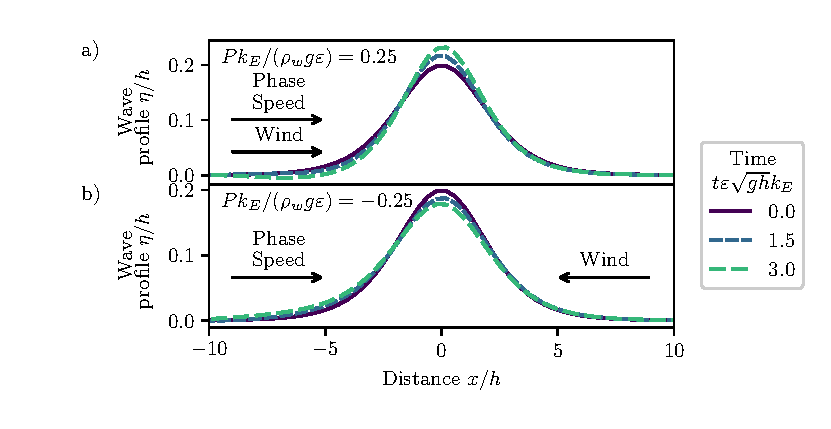
\includegraphics{Snapshots-Positive-Negative-Production.eps}
  \caption{
    Evolution of a solitary wave profile under
    \subref{fig:snapshots_solitary:a}
    onshore and
    \subref{fig:snapshots_solitary:b}
    offshore Jeffreys forcing.
    The nondimensional wave height $\eta/h$ is plotted for
    nondimensional distance $-10 \le x/h \le 10$.
    Results are shown for $\epsilon=0.1$, $\mu_E = 0.6$, and $\abs{P
    k_E/(\rho_w g \epsilon)} = 0.25$ nondimensional slow times $t
    \epsilon \sqrt{gh} k_E = 0$, $2$, and $4$, as indicated in the
    legend.
    The arrows denote the direction of wave propagation (phase speed) or
    wind direction.
  }\label{fig:snapshots_solitary}
\end{figure}

The snapshots of the wave profile $\eta/h$ in
\cref{fig:snapshots_solitary} qualitatively show how the wave shape
evolves over nondimensional time $t \epsilon \sqrt{g h} k_E$ when
plotted against the nondimensional distance $x/h$.
Both the onshore wind \subref{fig:snapshots_solitary:a} and offshore
wind \subref{fig:snapshots_solitary:b} begin from an identical,
symmetrical solitary wave profile at $t=0$ which would satisfy the
unforced KdV equation.
The onshore case \subref{fig:snapshots_solitary:a} demonstrates
marked, accelerating wave growth while the offshore wind
\subref{fig:snapshots_solitary:b} causes decay which slows over time.
Furthermore, the wind induces a horizontal asymmetry in the wave shape.
In both cases, the windward side of the wave becomes steeper (up to
\SI{8}{\percent} steeper for the time period shown) than the leeward
side.
Finally, while the front face of the wave shows only a moderate change in
slope, the rear face of the wave shows a qualitative difference between
the two wind directions.
Namely, the offshore wind raises the rear base of the wave relative to
its initial profile while an onshore wind depresses it, even forming a
small depression below the still water level.

\begin{figure}
  \centering
  { % Put \phantomsubcaption in their own group to prevent it from
    % affecting the main figure's numbering
    \phantomsubcaption{}\label{fig:statistics_solitary:a}
    \phantomsubcaption{}\label{fig:statistics_solitary:b}
    \phantomsubcaption{}\label{fig:statistics_solitary:c}
  }
  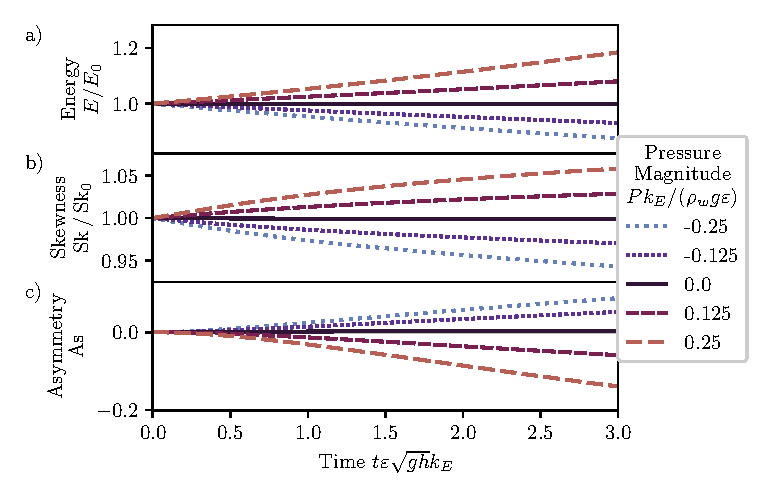
\includegraphics{Skew-Asymm-Production.eps}
  \caption{
    Shape statistics of a solitary profile under onshore and offshore
    Jeffreys forcing are shown for nondimensional slow time $t \epsilon
    \sqrt{gh} k_E \numrange{0}{4}$.
    The
    \subref{fig:statistics_solitary:a}
    height,
    \subref{fig:statistics_solitary:b}
    skewness normalized by the initial time, and
    \subref{fig:statistics_solitary:c}
    asymmetry are defined in
    \cref{eq:height_def,eq:shape_stats_def}.
    Results are shown for $\epsilon=0.1$, $\mu_E = 0.6$, and $P
    k_E/(\rho_w g \epsilon) = 0$, $\pm 0.125$, and $\pm 0.25$, as
    indicated in the legend.
    The solid black line corresponds to the unforced case, $P = 0$, and
    shows no growth or asymmetry and a constant, positive skewness.
  }\label{fig:statistics_solitary}
\end{figure}

In order to quantify the effect of wind on wave shape,
\cref{fig:statistics_solitary} shows shape statistics as functions of
the nondimensional slow time $t \epsilon \sqrt{g h} k_E$ for onshore
wind ($P k_E/(\rho_w g \epsilon) = 0.125$ and $0.25$), offshore wind ($P
k_E/(\rho_w g \epsilon) = -0.125$ and $-0.25$), and the unforced case
($P k_E/(\rho_w g \epsilon) = 0$).
We plot all cases for initial steepness $\epsilon = 0.1$ up to slow
time $t'_1 = 3$, corresponding to $4/\epsilon = 30$ wave periods.
We calculate the \subref{fig:statistics_solitary:a} wave height as
\begin{equation}
  H(t) = \max(\eta) - \min(\eta) \,.
  \label{eq:height_def}
\end{equation}
The height \subref{fig:statistics_solitary:a} begins at $H_0/h = 2
\epsilon = 0.2$ and shows the onshore wind
causing wave growth while the offshore wind causes decay, as was
observed in \cref{fig:snapshots_solitary}.
Again, the onshore wind causes faster growth than the offshore wind
causes decay as observed in \cref{fig:snapshots_solitary}.

We quantify wave shape by the third-order moments, skewness and
asymmetry.
The \subref{fig:statistics_solitary:b} skewness and
\subref{fig:statistics_solitary:c} asymmetry are
\begin{equation}
  \Sk \coloneqq \frac{\langle \eta^3 \rangle}{\langle \eta^2
  \rangle^{3/2}} \
  \qq{and}
  \As \coloneqq \frac{\langle \hilbert \Bqty{\eta^3} \rangle}{\langle
    \eta^2 \rangle^{3/2}} \,,
  \label{eq:shape_stats_def}
\end{equation}
with
\begin{equation}
  \langle f \rangle \coloneqq \frac{1}{L'_x} \int_{-L'_x/2}^{L'_x/2} f
  \dd{x}
\end{equation}
and $\hilbert$ the Hilbert transform.
Since this definition caries a factor of the
domain size $\sqrt{L'_x}$, we normalize by the initial skewness.
The onshore (offshore) causes the wave to become more (less) skewed over
time.
The skewness is nearly symmetric with respect to $\pm P$ about one.
The initial profile has zero asymmetry, and the unforced case
$P=0$ maintains zero asymmetry over time.
However, the onshore wind causes the asymmetry to become negative
corresponding to a tilting backwards, while the offshore wind increases
the asymmetry causing the wave to tilt forwards, as seen in
\cref{fig:snapshots_solitary}.
Notice that $\abs{\As}$ is larger for onshore winds than offshore winds.
The definitions of the skewness and asymmetry are insensitive to scaling
of the waveform $\eta \to \lambda \eta$, so this effect is not simply
caused by the wave's growth under an onshore wind.
Instead, over \SI{80}{\percent} of the discrepancy between $P>0$
and $P<0$ asymmetries arises from the left half of the wave.
This is consistent with the observation from
\cref{fig:snapshots_solitary} that the left side has a much more
apparent shape change.

\section{\label{sec:discussion} Discussion}

\subsection{\label{sec:press_mag} Wind Speed Estimation}
In \cref{sec:nondim}, we chose to nondimensionalize the pressure as
$P k_E/(\rho_w g) = \order{\epsilon}$, which corresponds to the
intermediate strength wind analyzed in \citet{zdyrski2020wind}.
Now, we will estimate the wind speed associated with such a pressure
magnitude to show that such a choice is reasonable.
First we need the growth rate of the energy $E$, which can be fit
numerically to
\begin{equation}
  E \coloneqq \rho_w g \int_{-\infty}^{\infty} {\eta'}_0^2 \dd{x}
  \propto \frac{1}{1 - \gamma' t'}
  \qq{with}
  \gamma' \coloneqq b \bqty{\frac{P k_E}{\rho_w g}}
  \,,
  \label{eq:actual_energy}
\end{equation}
and $b = 1.992 \pm \num{1e-4}$.
This is close to the analytic approximation for the decay time, giving
$b = 4/15$~(\eg{} eq.\ 72 of \citealp{zdyrski2019effects} with
$\mathcal{A}=1$, $\mathcal{B} = 3/2$, $\mathcal{C} = \mu_E/(6\epsilon) =
1$, $\mathcal{G} = (P k_E)/(2 \rho_w g)$, and $c_0 = H_0 = 2$).
This is consistent with the observation in
\cref{fig:snapshots_solitary,fig:statistics_solitary} that the energy
(and height) change accelerates for $P>0$ but decelerates for $P<0$.
Alternatively, we can approximate the energy growth rate from the KdVB
equation \cref{eq:kdvb_nondim} with the standard procedure
\citep[\eg][]{mei2005nonlinear} of multiplying by $\eta'_0$ and
integrating from $x'=-\infty$ to $\infty$:
\begin{equation}
  \pdv{t'_1} \int_{-\infty}^{\infty} {\eta'}_0^2 \dd{x}
  = \int_{-\infty}^{\infty} P' \pqty{\pdv{\eta'_0}{x'}}^2
  \dd{x} \,.
\end{equation}
Redimensionalizing gives the energy growth rate $\gamma$,
\begin{equation}
  \frac{\gamma}{c k_E} \coloneqq
  \frac{1}{c k_E E} \pdv{E}{t}
  = \frac{P k_E}{\rho_w g} \frac{\langle (\partial_x \eta)^2 \rangle}
    {\langle (k_E \eta)^2 \rangle}
  = \frac{1}{5} \frac{P k_E}{\rho_w g}
  \,,
  \label{eq:gamma_vs_P_solitary}
\end{equation}
with the phase speed $c = \sqrt{gh}$.
In the final equation, we evaluated the growth rate for the initial
solitary wave profile \cref{eq:initial_condition}.
Such a relationship between the surface pressure $p(x,t)$ and growth
rate holds generally for any form of pressure
forcing~\citep[\eg][]{peirson2008wind}.
Note that this is consistent with the growth rate found in
\cref{eq:actual_energy} for small times $\gamma t \ll 1$.

Additionally, \citet{jeffreys1925formation} theory relates this growth
rate to the wind speed $U_z$, measured at some height $z$, as
\begin{equation}
  \frac{\gamma}{\omega} = S_z \frac{\rho_a}{\rho_w}
    \pqty{\frac{U_z}{c}-1} \abs{\frac{U_z}{c}-1} \,.
  \label{eq:gamma_vs_u_jeffreys}
\end{equation}
Combining this with \cref{eq:gamma_vs_P_solitary} gives
\begin{equation}
  U_z = c \pqty{1 \pm \sqrt{\frac{1}{5} \abs{\frac{P k_E}{\rho_w g}}
    \frac{\rho_w}{\rho_a} \frac{1}{S_z}}} \,.
\end{equation}
Here, the $\pm$ corresponds to onshore ($+$) or offshore ($-$) winds.
Note that changing the wind direction (\ie{} sign of $Pk_E/(\rho_w g)$,
or $\pm$ sign) while holding the surface pressure magnitude
$\abs{Pk_E/(\rho_w g)}$ constant means $\abs{U_z}$ onshore will be
larger than $\abs{U_z}$ offshore.

\Citet{donelan2006wave} provides a parameterization for shallow water
waves that depends on airflow separation: $S_{\lambda/2} =
(ak)\bqty{4.91-3.98 H\Bqty{(ak)\bqty{(U_{\lambda/2}/c)^2-1} - 1}}$, with
$H$ the Heaviside function.
We can evaluate $U_z$ for the parameters used in \cref{sec:results}
($\epsilon=0.1$, $\mu_E = 0.6$, $Pk/(\rho_w g \epsilon) = 0.25$).
This yields a non-separated flow, $(ak)\bqty{(U_{\lambda/2}/c)^2-1} <
1$.
We choose $\lambda = \SI{20}{\meter}$ to give the wind speed at
$z=\SI{10}{\meter}$: $U_{10} = \SI{21}{\meter\per\second}$.
For reference, these parameters correspond to a depth of $h =
\SI{2.5}{\meter}$ and initial wave height $H_0 = \SI{0.5}{\meter}$.

\subsection{Physical Interpretation}
In \cref{sec:results}, we noted that the rear face of the waves in
\cref{fig:snapshots_solitary} showed marked shape differences between
onshore and offshore wind, while the front faces were rather similar.
This can be understood by considering the fluid velocity, which is
largely right-to-left in this co-moving frame.
When the water approaches the solitary wave from $x = +\infty$, it is
virtually unaffected by the pressure, since $p \propto \partial_x \eta$
is negligible far away from the wave.
Hence, the front face of the wave (the right side) is largely unaffected
by the pressure forcing.
For the onshore wind case, the water rising on the right side of the
wave encounters low air pressure, and the water descending on the left
hand side encounters high air pressure, both of which increase the
water's energy.
This additional kinetic energy causes the water flow to overshoot $z=0$
at the rear base of the wave, leading to the overshoot observed.
The opposite holds for the onshore wind, where wind removes kinetic energy
from the flow, so that the flow does not immediately return to the still
water level.
As discussed in \cref{sec:results}, this discrepancy between the front
and rear faces of the wave is also largely responsible for the variation
between onshore asymmetry and offshore asymmetry in
\cref{fig:statistics_solitary}.

\subsection{Comparison to Intermediate and Deep Water}
Here, we have coupled wind to waves in shallow water.
A previous study \citep{zdyrski2020wind} instead coupled wind and waves
in intermediate to deep water.
That study investigated the effect of wind on Stokes-like waves as
solitary waves are not possible.
However, qualitative agreement is still found between these two studies.
\Cref{fig:statistics_solitary} shows that, for a fixed time $t \neq 0$,
the asymmetry increases as the pressure $P$ increases.
We observed a similar trend for the corresponding Jeffreys pressure
profile in \figname{} 4(a) of \citet{zdyrski2020wind}, where the
harmonic phase $\beta$ is plotted against pressure magnitude $P$.
Note that $\As \propto -\sin{\beta}$, to leading order \citep[\cf
eq.\ 3.55 of][]{zdyrski2020wind}.

For this study, we investigated the effect of wind on periodic,
cnoidal-like waves, in direct analogy to the periodic, Stokes-like waves
of \citet{zdyrski2020wind}.
The pressure induced shape statistics were qualitatively similar to
those derived for solitary waves, so they are not shown here for
brevity.
Furthermore, we used a Jeffreys-type surface pressure profile to
couple wind and waves.
\Citet{zdyrski2020wind} utilized three different surface pressure
profiles: the same Jeffreys-type, a Miles-type which proved unphysical,
and a Generalized Miles (GM)-type wherein the pressure was proportional to
$\eta$ shifted by a distance parameter $\psi_P/k$.
When applied to shallow water, cnoidal-like waves, the GM profile
generates an asymmetry whose sign is consistent with
\citet{zdyrski2020wind}.
However, results for GM forcings were not included here since the GM
forcing is most applicable to periodic waves (\eg{} Stokes waves or
cnoidal waves), and it produces unphysical effects such as the growth of
higher harmonics under offshore winds.

\section{Conclusion}
Prior results~\citep{zdyrski2020wind} in intermediate and deep water
demonstrated that wind, acting though an $\eta$-dependent surface
pressure, can generate shape changes that become more pronounced in
shallow water.
This motivated the current work which used a multiple scales analysis to
couple weak wind with mild-slope long waves, \ie{} $H_0/h \sim (k_E h)^2
\sim P k/(\rho_w g) \ll 1$.
This derivation produced a KdV-Burgers equation governing the wave
profile $\eta$.
We utilized a symmetric solitary wave satisfying the unforced KdV
equation as our initial condition.
A third-order Runge Kutta solver determined the time-evolution of the
surface profile, and we extracted height, skewness, and asymmetry as
functions of time and pressure magnitude.
For onshore wind (positive $P$), wave height and skewness increased with
time while asymmetry decreased, with offshore wind producing opposite
effects.
Furthermore, these effects were enhance for strong pressures, reducing
to the unforced case for $P=0$.
The shape statistics found here show qualitative agreement with the
results in intermediate and deep water, and future work on periodic
shallow-water waves would allow a direct, quantitative comparison with
the periodic deep-water waves.
Declaration of Interests. The authors report no conflict of interest.

\appendix

% Bibliography
\bibliographystyle{jfm}
\bibliography{references}

\end{document}
